\subsection{Estudio Externo -- Análisis POAM}
\label{sec:estudio_externo}

\subsubsection{Marco Metodológico POAM}

El Perfil de Oportunidades y Amenazas del Medio (POAM) es una metLa Tabla \ref{tab:matriz_poam_completa} presenta la evaluación detallada de todas las variables del entorno externo consideradas en el análisis POAM, permitiendo identificar las oportunidades y amenazas más relevantes para MercadoLibre en el contexto latinoamericano.

\subsubsection{Resultados de la Evaluación POAM}logía de análisis estratégico que permite identificar y evaluar sistemáticamente los factores externos que pueden influir en el desempeño organizacional. Este análisis se desarrolla siguiendo siete pasos metodológicos secuenciales que aseguran una evaluación integral y objetiva del entorno externo de MercadoLibre \autocite{david2017}.

La metodología POAM facilita la transformación de factores cualitativos del entorno en evaluaciones cuantitativas que permiten la priorización estratégica y la toma de decisiones fundamentadas. El análisis integra perspectivas del modelo PESTEL con evaluaciones de impacto específicas para el contexto de comercio electrónico y servicios financieros en América Latina.

\subsubsection{Paso 1: Unidades de Análisis}

Para el análisis POAM de MercadoLibre se han identificado seis unidades de análisis críticas que abarcan los principales factores del entorno externo:

\begin{enumerate}
\item \textbf{Entorno Económico}: Factores macroeconómicos que afectan el poder adquisitivo, tasas de interés, inflación y estabilidad monetaria en los mercados de operación.
\item \textbf{Entorno Político}: Marco regulatorio, políticas gubernamentales, estabilidad institucional y regulaciones específicas del sector fintech y e-commerce.
\item \textbf{Entorno Tecnológico}: Innovaciones tecnológicas, infraestructura digital, adopción de nuevas tecnologías y capacidades de integración sistémica.
\item \textbf{Entorno Competitivo}: Dinámica de competencia, nuevos entrantes, productos sustitutos y rivalidad en el sector.
\item \textbf{Entorno Social-Cultural}: Cambios demográficos, hábitos de consumo, preferencias culturales y adopción digital por parte de los usuarios.
\item \textbf{Entorno Ambiental}: Sostenibilidad, responsabilidad ambiental y regulaciones medioambientales.
\end{enumerate}

\subsubsection{Paso 2: Variables por Unidad de Análisis}

\subsubsection{Entorno Económico}

El entorno económico abarca los factores macroeconómicos que influyen directamente en el poder adquisitivo de los consumidores y en la viabilidad financiera de las operaciones de MercadoLibre en los diferentes mercados latinoamericanos.

\begin{itemize}
\item \textbf{Capacidad Adquisitiva de la Población}: Evalúa el poder de compra real de los consumidores en los mercados objetivo, considerando ingresos disponibles, distribución del ingreso y tendencias de consumo. Una reducción en la capacidad adquisitiva impacta directamente las ventas en la plataforma y la demanda de servicios financieros.

\item \textbf{Niveles de Inflación Regional}: Analiza las tasas de inflación en los países de operación y su efecto en la estabilidad de precios de productos y servicios. La inflación elevada puede generar volatilidad en los precios de la plataforma y afectar la predictibilidad de los márgenes operativos.

\item \textbf{Tasas de Interés y Costo de Capital}: Examina las políticas monetarias de los bancos centrales y su impacto en el costo de financiamiento para MercadoLibre y sus usuarios. Las tasas de interés afectan tanto los costos de capital para expansión como la demanda de productos de crédito de Mercado Pago.

\item \textbf{Tipo de Cambio y Volatilidad Monetaria}: Evalúa la estabilidad cambiaria en los mercados de operación y su efecto en las operaciones transfronterizas, conversión de resultados financieros y competitividad de productos importados en la plataforma.
\end{itemize}

\subsubsection{Entorno Político}

El entorno político comprende el marco regulatorio, las políticas gubernamentales y la estabilidad institucional que afectan las operaciones de comercio electrónico y servicios financieros en América Latina.

\begin{itemize}
\item \textbf{Aranceles de Importación}: Analiza las políticas comerciales y arancelarias que afectan el costo y disponibilidad de productos importados en la plataforma. Los cambios arancelarios pueden impactar la competitividad de ciertos productos y la estructura de precios del marketplace.

\item \textbf{Legislación Interna de Comercio Electrónico}: Evalúa el marco legal que regula las actividades de comercio electrónico, incluyendo protección al consumidor, resolución de disputas, regulaciones de marketplace y responsabilidades de intermediación digital.

\item \textbf{Regulaciones Fintech y de Pagos Digitales}: Examina las regulaciones específicas para servicios financieros digitales, licencias requeridas para operar como entidad financiera, requisitos de capital y normativas de prevención de lavado de dinero que afectan las operaciones de Mercado Pago.

\item \textbf{Estabilidad Política Regional}: Considera la estabilidad institucional y la predictibilidad del marco regulatorio en los países de operación, factores que influyen en las decisiones de inversión y expansión a largo plazo.
\end{itemize}

\subsubsection{Entorno Tecnológico}

El entorno tecnológico abarca las innovaciones, infraestructura digital y capacidades tecnológicas disponibles en el ecosistema que pueden influir en la competitividad y capacidad de innovación de MercadoLibre.

\begin{itemize}
\item \textbf{Nuevas Tecnologías Emergentes (IA, Blockchain)}: Evalúa la disponibilidad y madurez de tecnologías emergentes como inteligencia artificial, machine learning, blockchain y computación cuántica que pueden generar nuevas oportunidades de diferenciación o disrupciones competitivas.

\item \textbf{Integración con Herramientas Antiguas}: Analiza los desafíos y oportunidades relacionados con la integración de nuevas tecnologías con sistemas legacy de vendedores, instituciones financieras y proveedores logísticos en el ecosistema.

\item \textbf{Infraestructura de Telecomunicaciones}: Examina la calidad y cobertura de la infraestructura de conectividad en los mercados objetivo, factor crítico para la adopción de servicios digitales y la experiencia del usuario en plataformas de e-commerce.

\item \textbf{Ciberseguridad y Protección de Datos}: Considera las amenazas de seguridad digital, regulaciones de protección de datos personales y los estándares de ciberseguridad requeridos para mantener la confianza del ecosistema y cumplir con regulaciones como LGPD en Brasil.
\end{itemize}

\subsubsection{Entorno Competitivo}

El entorno competitivo analiza la estructura de la industria, la intensidad de la competencia y la evolución de modelos de negocio que pueden afectar la posición competitiva de MercadoLibre.

\begin{itemize}
\item \textbf{Competencia Nacional Establecida}: Evalúa la presencia y fortaleza de competidores locales en cada mercado, incluyendo retailers tradicionales que han desarrollado capacidades digitales y marketplaces regionales que compiten directamente con MercadoLibre.

\item \textbf{Competencia Internacional (Amazon, Shopee)}: Analiza la estrategia de expansión y inversión de competidores globales en América Latina, considerando sus ventajas en recursos financieros, tecnología y experiencia en otros mercados emergentes.

\item \textbf{Público Objetivo y Segmentación}: Examina la evolución de los segmentos de clientes objetivo, incluyendo cambios demográficos, preferencias de consumo y la emergencia de nuevos segmentos como la economía digital y el comercio B2B.

\item \textbf{Nuevos Modelos de Negocio Disruptivos}: Considera la amenaza de modelos innovadores como super apps, social commerce, live commerce y plataformas especializadas que pueden capturar segmentos específicos del mercado o cambiar las expectativas de los usuarios.
\end{itemize}

\subsubsection{Entorno Social-Cultural}

El entorno social-cultural comprende los cambios demográficos, culturales y de comportamiento que influyen en la adopción de servicios digitales y las preferencias de consumo en América Latina.

\begin{itemize}
\item \textbf{Envejecimiento Poblacional}: Analiza el cambio demográfico hacia una población más madura en ciertos mercados, lo que representa oportunidades para segmentos con mayor poder adquisitivo y necesidades específicas de servicios financieros y productos especializados.

\item \textbf{Migración de Población a Zonas Urbanas}: Evalúa el proceso de urbanización en América Latina y su impacto en la concentración de usuarios potenciales en áreas con mejor infraestructura digital y logística, facilitando la penetración de servicios de e-commerce.

\item \textbf{Medios de Comunicación y Marketing Digital}: Examina la saturación de canales digitales de marketing, el aumento en costos de adquisición de clientes (CAC) y la necesidad de innovar en estrategias de comunicación para mantener la efectividad publicitaria.

\item \textbf{Adopción de Pagos Digitales}: Considera la aceleración en la adopción de medios de pago digitales, especialmente post-pandemia, y las oportunidades para expandir los servicios financieros de Mercado Pago en segmentos tradicionalmente no bancarizados.
\end{itemize}

\subsubsection{Entorno Ambiental}

El entorno ambiental abarca las consideraciones de sostenibilidad, responsabilidad ambiental y regulaciones medioambientales que influyen en las operaciones y reputación corporativa de MercadoLibre.

\begin{itemize}
\item \textbf{Políticas de Sostenibilidad Corporativa}: Evalúa las expectativas crecientes de stakeholders respecto a prácticas empresariales sostenibles y el impacto en la reputación corporativa y preferencias de consumidores conscientes del medio ambiente.

\item \textbf{Regulaciones Ambientales}: Analiza el marco regulatorio ambiental emergente que puede afectar operaciones logísticas, embalaje de productos y huella de carbono de las operaciones de e-commerce.

\item \textbf{Logística Verde y Reducción de Emisiones}: Examina las oportunidades y desafíos para implementar prácticas logísticas sostenibles, incluyendo vehículos eléctricos para entregas, optimización de rutas y empaques biodegradables.

\item \textbf{Responsabilidad Social Empresarial}: Considera las expectativas de contribución al desarrollo social y económico de las comunidades donde opera MercadoLibre, incluyendo programas de inclusión financiera y apoyo a emprendedores locales.
\end{itemize}

\subsubsection{Metodología de Evaluación POAM}

La evaluación se realiza mediante la asignación de valores de importancia (1--5) e impacto externo ($-3$ a $+3$) para cada variable:

\begin{itemize}
\item \textbf{Escala de Importancia}: 1 = Muy baja, 2 = Baja, 3 = Media, 4 = Alta, 5 = Muy alta
\item \textbf{Escala de Impacto}: $-3$ = Amenaza muy alta, $-2$ = Amenaza alta, $-1$ = Amenaza media, 0 = Factor neutro, $+1$ = Oportunidad media, $+2$ = Oportunidad alta, $+3$ = Oportunidad muy alta
\end{itemize}

La evaluación ponderada se calcula multiplicando la importancia por el impacto para cada variable analizada, permitiendo identificar los factores con mayor relevancia estratégica.

\subsubsection{Matriz POAM -- Perfil de Oportunidades y Amenazas}

\begin{table}[H]
\centering
\footnotesize
\begin{tabular}{|p{2.2cm}|p{2.8cm}|c|c|c|c|c|c|c|c|c|c|}
\hline
\multirow{2}{*}{\textbf{Unidad}} & \multirow{2}{*}{\textbf{Variables}} & \multirow{2}{*}{\textbf{Imp.}} & \multirow{2}{*}{\textbf{Impacto}} & \multirow{2}{*}{\textbf{Pond.}} & \multicolumn{7}{c|}{\textbf{Escala de Evaluación}} \\
\cline{6-12}
& & & & & \textbf{-15} & \textbf{-10} & \textbf{-5} & \textbf{0} & \textbf{5} & \textbf{10} & \textbf{15} \\
\hline
\multirow{4}{*}{\makecell{Entorno\\Económico}} 
& Capacidad Adquisitiva & 4 & -2 & -8 & \multicolumn{1}{c|}{} & \multicolumn{1}{c|}{\textbullet} & \multicolumn{1}{c|}{} & \multicolumn{1}{c|}{} & \multicolumn{1}{c|}{} & \multicolumn{1}{c|}{} & \\
\cline{2-12}
& Precios & 5 & 2 & 10 & \multicolumn{1}{c|}{} & \multicolumn{1}{c|}{} & \multicolumn{1}{c|}{} & \multicolumn{1}{c|}{} & \multicolumn{1}{c|}{} & \multicolumn{1}{c|}{\textbullet} & \\
\cline{2-12}
& Tasas de Interés & 3 & 1 & 3 & \multicolumn{1}{c|}{} & \multicolumn{1}{c|}{} & \multicolumn{1}{c|}{} & \multicolumn{1}{c|}{} & \multicolumn{1}{c|}{\textbullet} & \multicolumn{1}{c|}{} & \\
\cline{2-12}
& Tipo de Cambio & 4 & -1 & -4 & \multicolumn{1}{c|}{} & \multicolumn{1}{c|}{} & \multicolumn{1}{c|}{\textbullet} & \multicolumn{1}{c|}{} & \multicolumn{1}{c|}{} & \multicolumn{1}{c|}{} & \\
\hline
\multirow{3}{*}{\makecell{Entorno\\Político}} 
& Aranceles de Importación & 3 & -1 & -3 & \multicolumn{1}{c|}{} & \multicolumn{1}{c|}{} & \multicolumn{1}{c|}{\textbullet} & \multicolumn{1}{c|}{} & \multicolumn{1}{c|}{} & \multicolumn{1}{c|}{} & \\
\cline{2-12}
& Legislación Interna & 3 & 2 & 6 & \multicolumn{1}{c|}{} & \multicolumn{1}{c|}{} & \multicolumn{1}{c|}{} & \multicolumn{1}{c|}{} & \multicolumn{1}{c|}{} & \multicolumn{1}{c|}{\textbullet} & \\
\cline{2-12}
& Regulación Fintech & 5 & 3 & 15 & \multicolumn{1}{c|}{} & \multicolumn{1}{c|}{} & \multicolumn{1}{c|}{} & \multicolumn{1}{c|}{} & \multicolumn{1}{c|}{} & \multicolumn{1}{c|}{} & \textbullet \\
\hline
\multirow{3}{*}{\makecell{Entorno\\Tecnológico}} 
& Nuevas Tecnologías & 3 & 0 & 0 & \multicolumn{1}{c|}{} & \multicolumn{1}{c|}{} & \multicolumn{1}{c|}{} & \multicolumn{1}{c|}{\textbullet} & \multicolumn{1}{c|}{} & \multicolumn{1}{c|}{} & \\
\cline{2-12}
& Integración Herramientas & 5 & 0 & 0 & \multicolumn{1}{c|}{} & \multicolumn{1}{c|}{} & \multicolumn{1}{c|}{} & \multicolumn{1}{c|}{\textbullet} & \multicolumn{1}{c|}{} & \multicolumn{1}{c|}{} & \\
\cline{2-12}
& Ciberseguridad & 5 & 1 & 5 & \multicolumn{1}{c|}{} & \multicolumn{1}{c|}{} & \multicolumn{1}{c|}{} & \multicolumn{1}{c|}{} & \multicolumn{1}{c|}{\textbullet} & \multicolumn{1}{c|}{} & \\
\hline
\multirow{4}{*}{\makecell{Entorno\\Competitivo}} 
& Competencia Nacional & 5 & 2 & 10 & \multicolumn{1}{c|}{} & \multicolumn{1}{c|}{} & \multicolumn{1}{c|}{} & \multicolumn{1}{c|}{} & \multicolumn{1}{c|}{} & \multicolumn{1}{c|}{\textbullet} & \\
\cline{2-12}
& Competencia Internacional & 3 & 1 & 3 & \multicolumn{1}{c|}{} & \multicolumn{1}{c|}{} & \multicolumn{1}{c|}{} & \multicolumn{1}{c|}{} & \multicolumn{1}{c|}{\textbullet} & \multicolumn{1}{c|}{} & \\
\cline{2-12}
& Público Objetivo & 4 & 3 & 12 & \multicolumn{1}{c|}{} & \multicolumn{1}{c|}{} & \multicolumn{1}{c|}{} & \multicolumn{1}{c|}{} & \multicolumn{1}{c|}{} & \multicolumn{1}{c|}{} & \textbullet \\
\cline{2-12}
& Modelos Disruptivos & 4 & -2 & -8 & \multicolumn{1}{c|}{} & \multicolumn{1}{c|}{\textbullet} & \multicolumn{1}{c|}{} & \multicolumn{1}{c|}{} & \multicolumn{1}{c|}{} & \multicolumn{1}{c|}{} & \\
\hline
\multirow{4}{*}{\makecell{Entorno\\Social-Cultural}} 
& Envejecimiento Poblacional & 4 & 3 & 12 & \multicolumn{1}{c|}{} & \multicolumn{1}{c|}{} & \multicolumn{1}{c|}{} & \multicolumn{1}{c|}{} & \multicolumn{1}{c|}{} & \multicolumn{1}{c|}{} & \textbullet \\
\cline{2-12}
& Migración a Zonas Urbanas & 4 & 2 & 8 & \multicolumn{1}{c|}{} & \multicolumn{1}{c|}{} & \multicolumn{1}{c|}{} & \multicolumn{1}{c|}{} & \multicolumn{1}{c|}{} & \multicolumn{1}{c|}{\textbullet} & \\
\cline{2-12}
& Medios de Comunicación & 5 & -2 & -10 & \multicolumn{1}{c|}{} & \multicolumn{1}{c|}{\textbullet} & \multicolumn{1}{c|}{} & \multicolumn{1}{c|}{} & \multicolumn{1}{c|}{} & \multicolumn{1}{c|}{} & \\
\cline{2-12}
& Adopción Digital & 5 & 3 & 15 & \multicolumn{1}{c|}{} & \multicolumn{1}{c|}{} & \multicolumn{1}{c|}{} & \multicolumn{1}{c|}{} & \multicolumn{1}{c|}{} & \multicolumn{1}{c|}{} & \textbullet \\
\hline
\multirow{2}{*}{\makecell{Entorno\\Ambiental}} 
& Sostenibilidad & 3 & 0 & 0 & \multicolumn{1}{c|}{} & \multicolumn{1}{c|}{} & \multicolumn{1}{c|}{} & \multicolumn{1}{c|}{\textbullet} & \multicolumn{1}{c|}{} & \multicolumn{1}{c|}{} & \\
\cline{2-12}
& Responsabilidad Social & 3 & 1 & 3 & \multicolumn{1}{c|}{} & \multicolumn{1}{c|}{} & \multicolumn{1}{c|}{} & \multicolumn{1}{c|}{} & \multicolumn{1}{c|}{\textbullet} & \multicolumn{1}{c|}{} & \\
\hline
\end{tabular}
\caption{Matriz POAM -- Perfil de Oportunidades y Amenazas MercadoLibre}
\label{tab:matriz_poam_completa}
\end{table}

La Tabla \ref{tab:matriz_poam_completa} presenta la evaluación detallada de todas las variables del entorno externo consideradas en el análisis POAM, permitiendo identificar las oportunidades y amenazas más relevantes para MercadoLibre \autocite{david2017}.

\subsubsection{Resultados Consolidados por Unidad de Análisis}

\begin{table}[H]
\centering
\begin{tabular}{|l|c|c|}
\hline
\textbf{Unidad de Análisis} & \textbf{Ponderación Total} & \textbf{Clasificación} \\
\hline
Entorno Social-Cultural & +25 & Oportunidad Significativa \\
\hline
Entorno Político & +18 & Oportunidad Significativa \\
\hline
Entorno Competitivo & +17 & Oportunidad Significativa \\
\hline
Entorno Tecnológico & +5 & Oportunidad Menor \\
\hline
Entorno Económico & +1 & Factor Neutro \\
\hline
Entorno Ambiental & +3 & Oportunidad Menor \\
\hline
\end{tabular}
\caption{Evaluación Ponderada por Unidad de Análisis -- POAM}
\label{tab:resultados_poam}
\end{table}

La Tabla \ref{tab:resultados_poam} consolida los resultados ponderados por cada unidad de análisis, mostrando que el entorno externo presenta oportunidades significativas en los aspectos social-culturales, políticos y competitivos \autocite{porter1985}.

\subsubsection{Análisis e Interpretación de Resultados POAM}

\paragraph{Principales Oportunidades Identificadas}

\begin{enumerate}
\item \textbf{Regulación Fintech Favorable (Ponderada: +15)}: Los marcos regulatorios pro-inclusión financiera en Brasil, México y Colombia facilitan la expansión de servicios de Mercado Pago y el desarrollo de nuevos productos financieros.

\item \textbf{Adopción Digital Acelerada (Ponderada: +15)}: El crecimiento en la adopción de pagos digitales y comercio electrónico en América Latina presenta oportunidades significativas de expansión de base de usuarios.

\item \textbf{Migración Urbana y Público Objetivo (Ponderada: +12)}: La concentración poblacional en zonas urbanas y la evolución demográfica favorecen la penetración de servicios digitales.

\item \textbf{Envejecimiento Poblacional (Ponderada: +12)}: El cambio demográfico crea nuevos segmentos de mercado con mayor poder adquisitivo y necesidades específicas de servicios financieros.

\item \textbf{Competencia Nacional (Ponderada: +10)}: La fragmentación de competidores locales permite oportunidades de consolidación y adquisición estratégica.
\end{enumerate}

\subsubsection{Principales Amenazas Identificadas}

\begin{enumerate}
\item \textbf{Saturación de Medios de Comunicación (Ponderada: -10)}: El incremento en costos de marketing digital y la saturación publicitaria afectan la eficiencia de adquisición de clientes.

\item \textbf{Reducción de Capacidad Adquisitiva (Ponderada: -8)}: Las presiones inflacionarias y la volatilidad económica regional impactan el poder de compra de los consumidores.

\item \textbf{Modelos de Negocio Disruptivos (Ponderada: -8)}: La entrada de competidores con modelos innovadores (como super apps asiáticas) representa amenazas al modelo tradicional de marketplace.

\item \textbf{Volatilidad Cambiaria (Ponderada: -4)}: Las fluctuaciones monetarias en mercados clave afectan la rentabilidad de operaciones transfronterizas.

\item \textbf{Aranceles de Importación (Ponderada: -3)}: Los cambios en políticas comerciales pueden impactar los costos de productos importados en la plataforma.
\end{enumerate}

\paragraph{Estrategias de Aprovechamiento y Mitigación}

\textbf{Para Oportunidades Principales:}
\begin{itemize}
\item Acelerar inversión en cumplimiento regulatorio y obtención de licencias fintech
\item Desarrollar productos específicos para segmentos demográficos emergentes
\item Implementar estrategias de adquisición de competidores locales fragmentados
\item Expandir servicios de inclusión financiera aprovechando marcos regulatorios favorables
\end{itemize}

\paragraph{Para Amenazas Principales:}
\begin{itemize}
\item Diversificar canales de marketing y optimizar eficiencia de CAC
\item Implementar estrategias de pricing dinámico sensible a condiciones económicas
\item Desarrollar capacidades de innovación interna para anticipar disrupciones
\item Establecer coberturas financieras para mitigar riesgo cambiario
\end{itemize}

\paragraph{Cuadro de Mando Integral}

El Cuadro de Mando Integral (Balanced Scorecard) representa una herramienta estratégica fundamental que permite traducir la visión y estrategia de MercadoLibre en un conjunto coherente de indicadores de desempeño. Esta metodología facilita la alineación organizacional y el seguimiento sistemático del progreso hacia los objetivos estratégicos, integrando perspectivas financieras y no financieras en un marco de gestión integral.

\begin{table}[H]
    \centering
    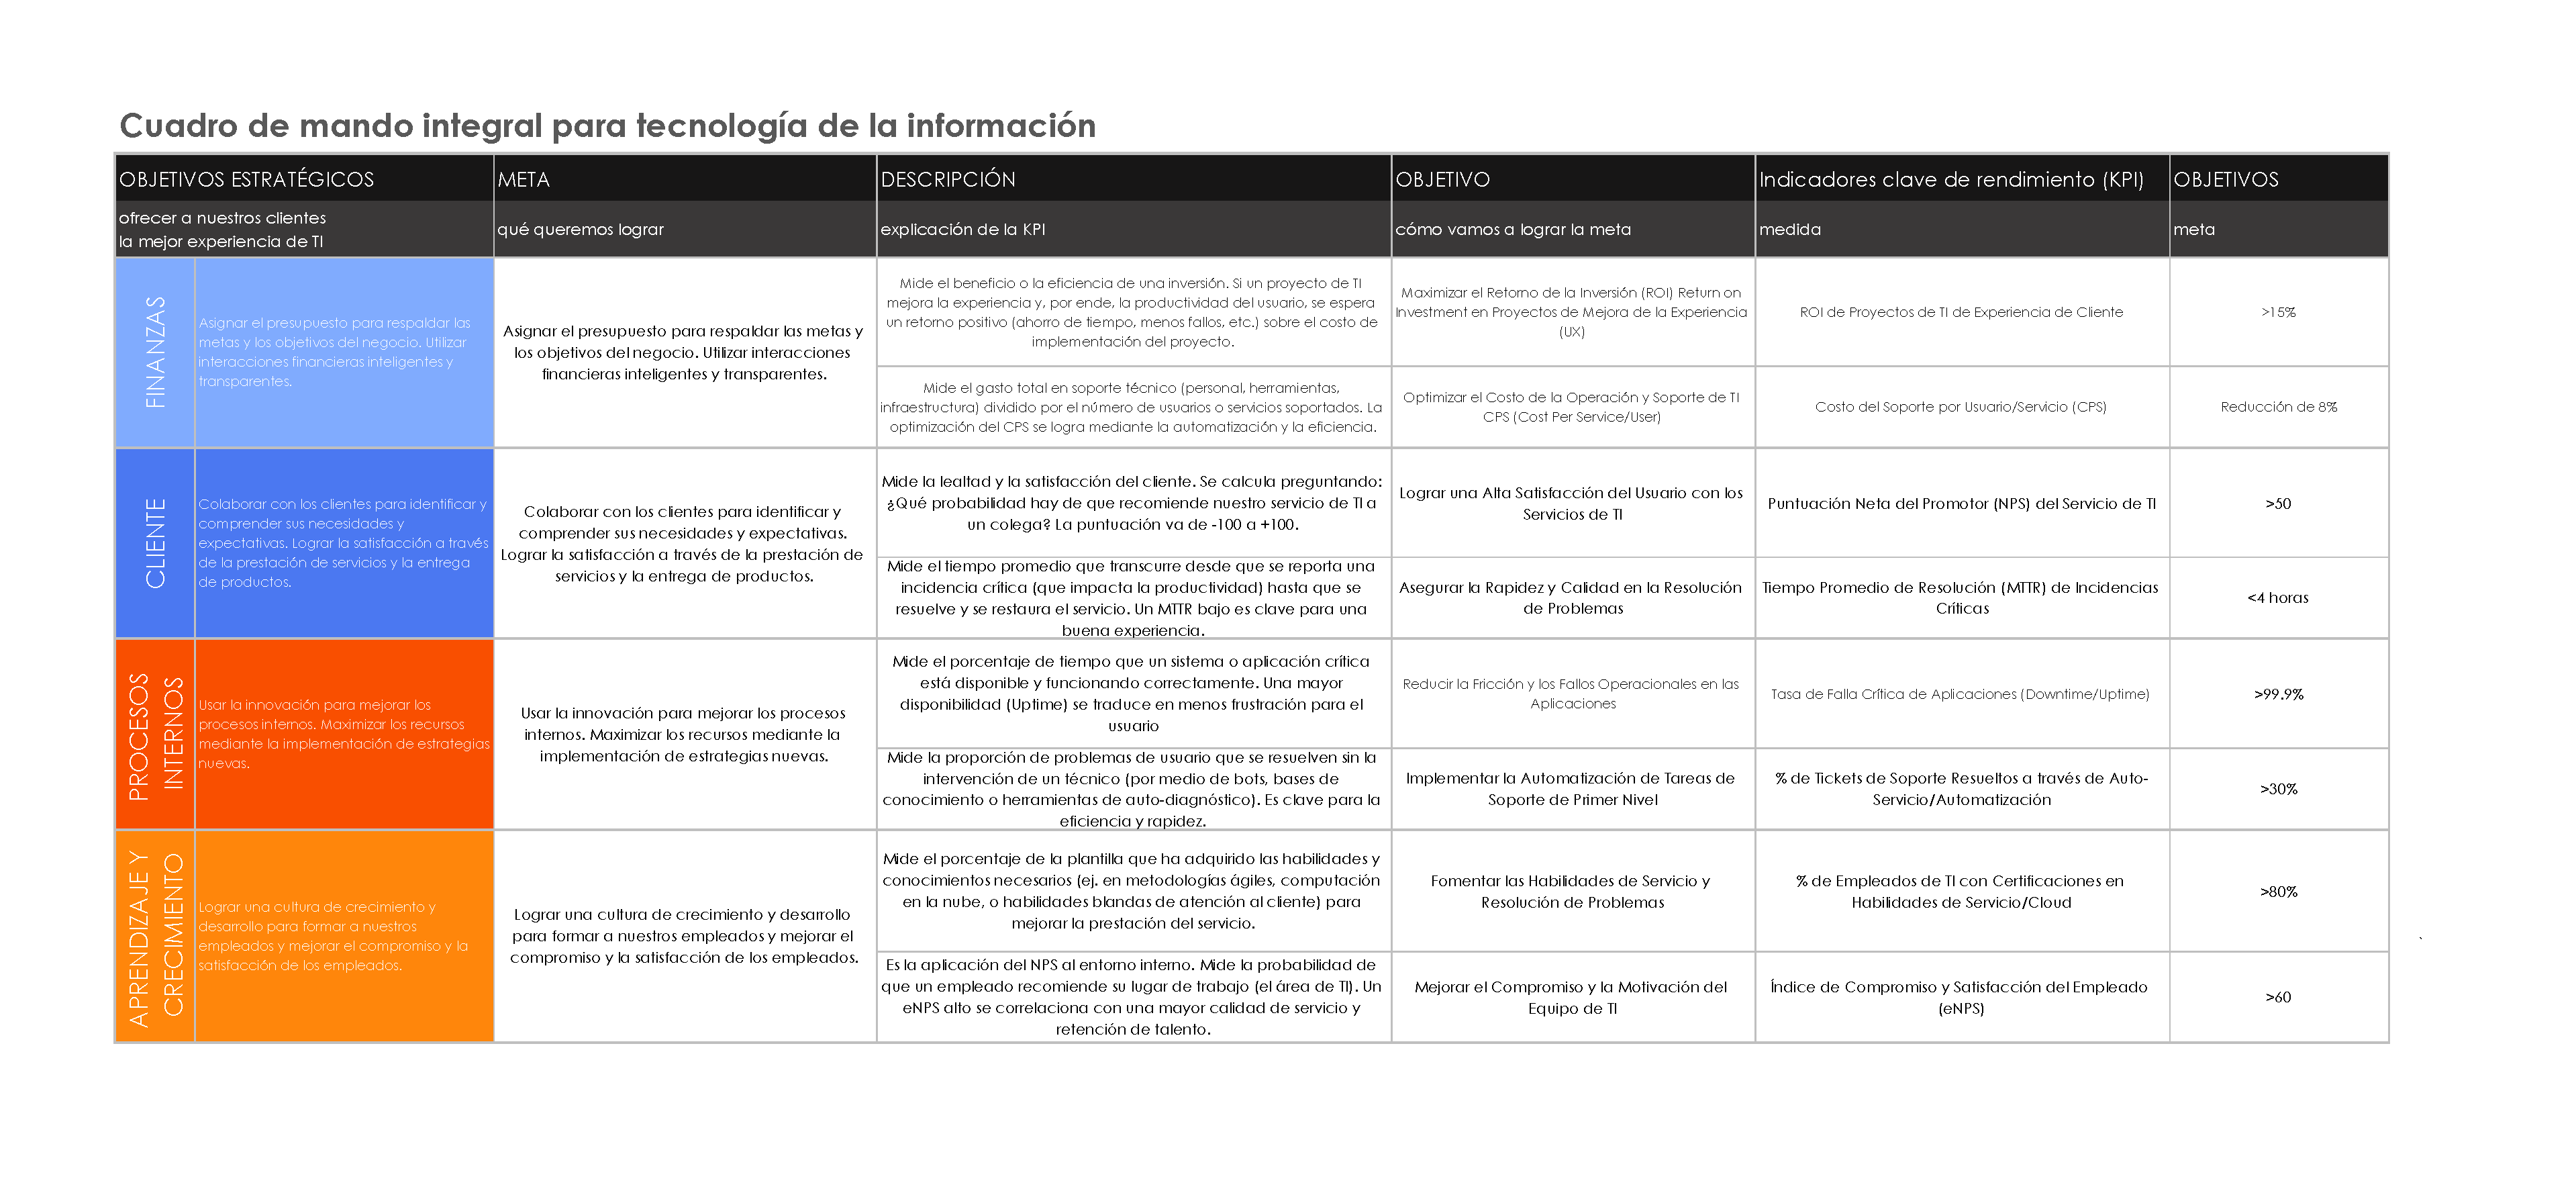
\includegraphics[width=\linewidth, height=0.8\textheight, keepaspectratio]{sections/Cuadro_Mando_Mercado_Libre.pdf}
    \caption{Cuadro de Mando Integral MercadoLibre}
    \label{tab:cuadro_mando_integral}
\end{table}

La Tabla \ref{tab:cuadro_mando_integral} presenta el Cuadro de Mando Integral diseñado específicamente para MercadoLibre, estructurado en las cuatro perspectivas clásicas del modelo: Financiera, Cliente, Procesos Internos, y Aprendizaje y Crecimiento. Este marco estratégico permite monitorear tanto los resultados operativos como los inductores de valor futuro, garantizando una gestión equilibrada entre objetivos de corto y largo plazo.

\paragraph{Síntesis del Análisis POAM}

El análisis POAM revela un entorno externo predominantemente favorable para MercadoLibre, con oportunidades significativas concentradas en regulación fintech y adopción digital. Las principales amenazas se relacionan con presiones de marketing y volatilidad económica, factores que requieren estrategias de mitigación específicas pero no comprometen la viabilidad del modelo de negocio.

La evaluación ponderada indica que los factores positivos superan significativamente a los negativos, sugiriendo un contexto estratégico propicio para la expansión y consolidación de la posición competitiva en el mercado latinoamericano de comercio electrónico y servicios financieros \autocite{porter1985}.
